\documentclass{article}
\usepackage{times}
\usepackage[nohead,bottom=3cm,top=2cm,a4paper]{geometry}
\usepackage{xcolor}
\usepackage{graphicx}
\usepackage[nswissgerman]{babel}
\usepackage{listings}
\usepackage{blindtext}
\usepackage{lipsum}
\usepackage{tikz}
\usetikzlibrary{positioning}
\usepackage{amssymb}    % math symbols
\usepackage{amsmath}    % math symbols
\graphicspath{ {./results/} }
\usetikzlibrary{shadows,matrix} % Shadows for nodes
\usetikzlibrary{arrows.meta}
\title{Report aus dem Projekt sensor Cube}
\author{von Ugur Turhal, Berkan Kurt \& Silvan Lenzlinger}
\begin{document}
\maketitle
\abstract{Dieses Report Dokument ist im Rahmen der Vorlesung, Rechenarchitektur \& vertrauenwürdiges Rechnen entstanden. Das Ziel war ein 4 x 4 x 4  Kubus zu löten. Diesen mit einem digitalen Luftfeuchtigskeits- \& Temperatursensor zu verbinden. Dieser soll anhand der idealen Luftfeuchtigkeit und der richtigen Temperatur, für den Schlaf, erreicht ist, spezifische Muster ausgeben.}
%%%%
\section{Einleitung}
Wir haben dieses Projekt gewählt, da

\section{Aufteilung}

\section{Jigs}
 
\section{Sammeln der Daten}
\paragraph{Daten}
\begin{center}
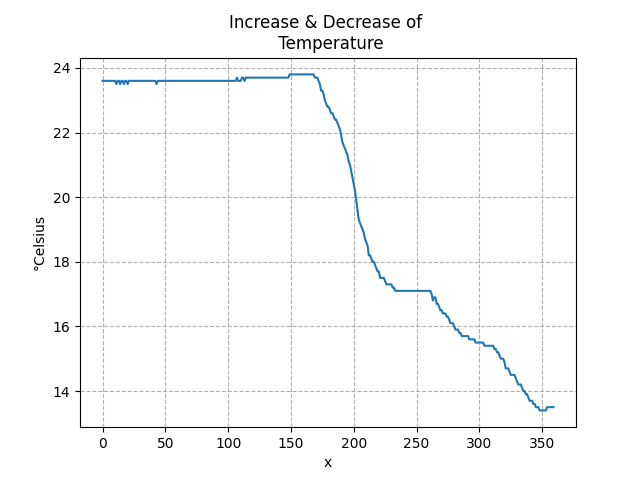
\includegraphics[width=0.49\textwidth]{plot.png}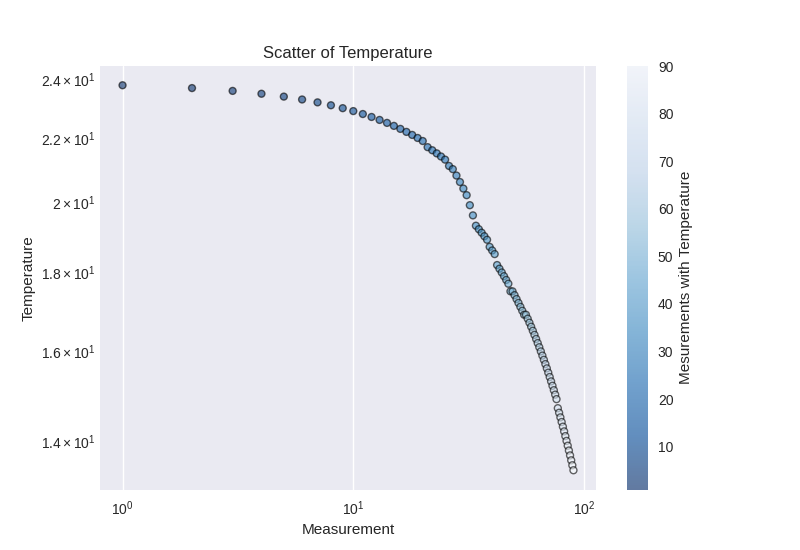
\includegraphics[width=0.53\textwidth]{scatter.png}
\end{center}

\begin{center}
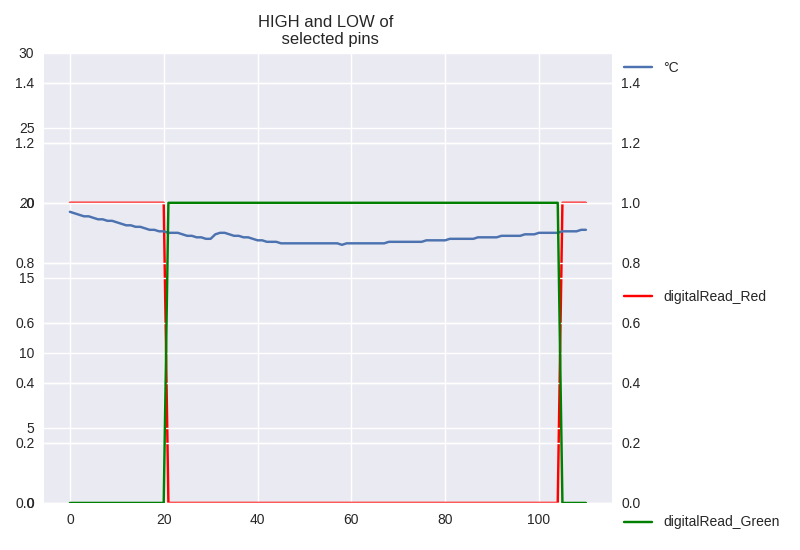
\includegraphics[width=0.53\textwidth]{digitalRead.png}
\end{center}

\section{Erkenntnisse durch die Daten}

\section{Umsetzung}

\tikzset{darkstyle/.style={circle,draw,fill=gray!40}}
\begin{figure}[h]
\centering
\begin{tikzpicture}
\begin{scope}[every node/.style={circle,thick,draw,fill=gray!40,level distance=200mm,}]
    \node (D48) at (0,0) {D48};
    \node (D46) at (2,0) {D46};
    \node (D44) at (4,0) {D44};
    \node (D42) at (6,0) {D42};
    
    \node (D46) at (2,0) {D46};
    \node (D44) at (4,0) {D44};
    \node (D42) at (6,0) {D42};
    
    \node (D40) at (0,-2) {D40};
    \node (D38) at (2,-2)  {D38};
    \node (D36) at (4,-2) {D36};
    \node (D34) at (6,-2) {D34};
    
    \node (D32) at (0,-4) {D32};
    \node (D30) at (2,-4)  {D30};
    \node (D28) at (4,-4) {D28};
    \node (D26) at (6,-4) {D26};
    
    \node (D24) at (0,-6) {D24};
    \node (D22) at (2,-6)  {D22};
    \node (A5) at (4,-6) {A5};
    \node (A4) at (6,-6) {A4};
    
\end{scope}

\begin{scope}[>={Stealth[black]},
              every node/.style={fill=gray!40,circle,thick},
              every edge/.style={draw=red,very thick}]
     \draw [color=red!100,->,line width=1] (A4) -- (A5);
     \draw [color=red!100,->,line width=1] (A5) -- (D22);
     \draw [color=red!100,->,line width=1] (D22) -- (D24);
     \draw [color=red!100,->,line width=1] (D24) -- (D32);
     \draw [color=red!100,->,line width=1] (D32) -- (D40);
     \draw [color=red!100,->,line width=1] (D40) -- (D48);
     
     \draw [color=red!100,->,line width=1] (D48) -- (D46);
     
     \draw [color=red!100,->,line width=1] (D46) -- (D38);
     \draw [color=red!100,->,line width=1] (D38) -- (D30);
     \draw [color=red!100,->,line width=1] (D30) -- (D22);
     
     \draw [color=red!100,->,line width=1] (D46) -- (D44);
     \draw [color=red!100,<-,line width=1] (D44) -- (D36);
     \draw [color=red!100,<-,line width=1] (D36) -- (D28);
     \draw [color=red!100,<-,line width=1] (D28) -- (A5);
     
     \draw [color=red!100,->,line width=1] (D44) -- (D42);
     \draw [color=red!100,->,line width=1] (D42) -- (D34);
     \draw [color=red!100,->,line width=1] (D34) -- (D26);
     \draw [color=red!100,->,line width=1] (D26) -- (A4);
   
\end{scope}

\end{tikzpicture}
\end{figure}

\section{Resultat}

\section{Evaluation des Resultats}

\section{Gewonnene Erkentnisse}

\section{Aufbau des Cubes}

\section{Danksagung}

%%%%


%%%%




\end{document}
